\section{Алгоритм на основе нисходящего анализа}

GLL~\cite{Grigorev:2017:CPQ:3166094.3166104}

Другие реализации~\cite{MEDEIROS201975}

\subsection{Нисходящий синтаксический анализ}

Рекурсивный спуск, LL, таблицы, неоднозначности, левая рекурсия.

\subsubsection{Рекурсивный спуск}

\begin{example}
Постороим функцию рекурсивного спуска для продукции $S \rightarrow aSbS$.

\begin{algorithm}
  \floatname{algorithm}{Listing}
\begin{algorithmic}[1]
\caption{Функция рекурсивного спуска}
\Function{S}{$hd'$, $tl'$}
    \State{$res = \{\}$}
    
    \If{$hd' = a$}
        \State{$res = $ S($tl'$)}
        \State{\textbf{else} $error$}
    \EndIf
      
    \If{head($res$) = $b$}
        \State{$res = $ S(tail($res$))}
        \State{\textbf{else} $error$}
    \EndIf
    
    \State \Return $res$
\EndFunction

\end{algorithmic}
\end{algorithm}
\end{example}

Если возвращаеммое значение этой функции пусто, то разбор завершился успехом.

\subsubsection{LL(k)-алгоритм синтаксического анализа}

LL(k) --- алгоритм синтаксического анализа --- нисходящий анализ без отката, но с предпросмотром. 
Решение о том, какую продукцию применять, принимается на основании k следующих за текущим символом. 
Временная сложность алгоритма $O(n)$, где $n$~--- длина слова. 

Алгоритм использует входной буфер, стек для хранения промежуточных данных и таблицу анализатора, которая управляет процессом разбора. 
В ячейке таблицы указано правило, которое нужно применять, если рассматривается нетерминал $A$, а следующие k символов строки~--- $t_{1} \dots t_{k}$. 
Также в таблице выделена отдельная колонка для $\$$~--- маркера конца строки. 

\begin{center}
  \begin{tabular}{ c || c | c | c | c }
             & $\dots$ & $t_{1} \dots t_{k}$ & $\dots$ & $\$$ \\ \hline  
    $\dots$  & $\dots$ & $\dots$ & $\dots$ & $\dots$ \\ \hline  
    $A$  & $\dots$ & $A \to \alpha$ & $\dots$ & $\dots$ \\ \hline  
    $\dots$  & $\dots$ & $\dots$ & $\dots$ & $\dots$ 
  \end{tabular}  
\end{center}

Для построения таблицы вычисляются множества $\first[k]$ и $\follow[k]$. Идейно их можно понимать, как первые или последующие $k$ символов в результирующем выводе, при использовании нетерминала $A$. Данную мысль хорошо иллюстрирует рисунок:

\begin{center}
    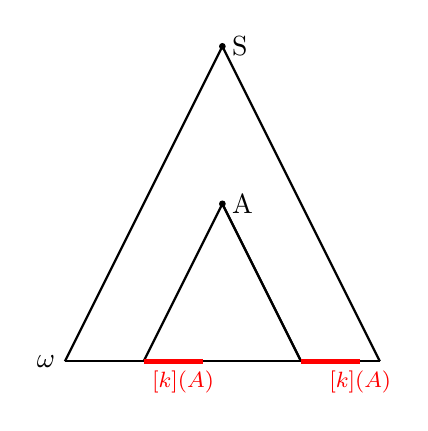
\begin{tikzpicture}
        \draw[black, thick] (0,0) -- (2,4);
        \draw[black, thick] (2,4) -- (4,0);
        \draw[black, thick] (1,0) -- (2,2);
        \draw[black, thick] (2,2) -- (3,0);
        \draw[black, thick] (2,2) -- (3,0);
        \draw[black, thick] (0,0) -- (1,0);
        \draw[red, ultra thick] (1,0) -- (1.75,0);
        \draw[black, thick] (1.75,0) -- (3,0);
        \draw[red, ultra thick] (3,0) -- (3.75,0);
        \draw[black, thick] (3.75,0) -- (4,0);
        \filldraw[black] (2,4) circle (1pt) node[anchor=west] {S};
        \filldraw[black] (2,2) circle (1pt) node[anchor=west] {A};
        \filldraw[black] (0,0) circle (0pt)
        node[anchor=east] {\textbf{$\omega$}};
        \filldraw[red] (1.5,0) circle (0pt)
        node[anchor=north] {\footnotesize $\first[k](A)$};
        \filldraw[red] (3.75,0) circle (0pt)
        node[anchor=north] {\footnotesize $\follow[k](A)$};
    \end{tikzpicture}
\end{center}

Определим их формально:

\begin{definition}
  Пусть $G = \langle N, \Sigma, P, S \rangle$~--- КС-грамматика. Множество $\first[k]$ определено для сентециальной формы $\alpha$ следующим образом:   
  \[ \first[k](\alpha) = \{ \omega \in \Sigma^* \mid \alpha \derives{} \omega \text{ и } |\omega| < k \text{ либо } \exists \beta: \alpha \derives{} \omega \beta \text{ и } |\omega| = k \} \text{, где } \alpha, \beta \in (N \cup \Sigma)^* \]
\end{definition}

\begin{definition}
  Пусть $G = \langle N, \Sigma, P, S \rangle$~--- КС-грамматика. Множество $\follow[k]$ определено для сентециальной формы $\beta$ следующим образом:
  \[\follow[k](\beta) = \{ \omega \in \Sigma^* \mid \exists \gamma, \alpha: S \derives{} \gamma \beta \alpha \text{ и } \omega \in \first[k](\alpha) \} \]
\end{definition}

В частном случае для $k = 1$: 

\[ \first(\alpha) = \{ a \in \Sigma \mid \exists \gamma \in (N \cup \Sigma)^*: \alpha \derives{} a \gamma \} \text{, где } \alpha \in (N \cup \Sigma)^* \]

\[ \follow(\beta) = \{ a \in \Sigma \mid \exists \gamma, \alpha \in (N \cup \Sigma)^* : S \derives{} \gamma \beta a \alpha \} \text{, где } \beta \in (N \cup \Sigma)^*  \]

Множество $\first$ можно вычислить, пользуясь следующими соотношениями:  

\begin{itemize}
  \item $\first(a \alpha) = \{a\}, a \in \Sigma, \alpha \in (N \cup \Sigma)^* $
  \item $\first(\varepsilon) = \{\varepsilon\}$
  \item $\first(\alpha \beta) = \first(\alpha) \cup (\first(\beta) \text{, если } \varepsilon \in \first(\alpha))$
  \item $\first(A) = \first(\alpha) \cup \first(\beta) \text{, если в грамматике есть правило } A \to \alpha \mid\beta$
\end{itemize}

Алгоритм для вычисления множества $\follow$: 

\begin{itemize}
  \item Положим $\follow(X) = \varnothing, \forall X \in N$
  \item $\follow(S) = \follow(S) \cup \{\$\} \text{, где } S \text{--- стартовый нетерминал}$
  \item Для всех правил вида $A \to \alpha X \beta: \follow(X) = \follow(X) \cup (\first(\beta) \setminus \{\varepsilon\} )$
  \item Для всех правил вида $A \to \alpha X \text{ и } A \to \alpha X \beta \text{, где } \varepsilon \in \first(\beta): \follow(X) = \follow(X) \cup \follow(A)$
  \item Последние два пункта применяются пока есть что добавлять в строящиеся множества. 
\end{itemize}

Пример множеств $\first$ для нетерминалов следующей грамматики: 

\begin{multicols}{2}
\begin{align*}
  S  &\to a S' \\ 
  S' &\to A b B S' \mid \varepsilon \\ 
  A  &\to a A' \mid \varepsilon \\ 
  A' &\to b \mid a \\ 
  B  &\to c \mid \varepsilon
\end{align*}

\columnbreak
    
\begin{align*}
  \first(S)  &= \{ a \} \\
  \first(A)  &= \{ a, \varepsilon \} \\ 
  \first(A') &= \{ a, b \} \\
  \first(B)  &= \{ c, \varepsilon \} \\
  \first(S') &= \{ a, b, \varepsilon \}  
\end{align*}
\end{multicols}

Пример множеств $\follow$ для нетерминалов следующей грамматики:

\begin{multicols}{2}
\begin{align*}
  S  &\to a S' \\ 
  S' &\to A b B S' \mid \varepsilon \\ 
  A  &\to a A' \mid \varepsilon \\ 
  A' &\to b \mid a \\ 
  B  &\to c \mid \varepsilon
\end{align*}

\columnbreak
    
\begin{align*}
  \follow(S)  &= \{ \$ \} & \\
  \follow(S') &= \{ \$ \} &(S \to a S')\\
  \follow(A)  &= \{ b \}  &(S' \to A b B S') \\ 
  \follow(A') &= \{ b \}  &(A \to a A')\\
  \follow(B)  &= \{ a, b, \$ \} &(S' \to A b B S', \varepsilon \in \first(S'))
\end{align*}  
\end{multicols}

Таблица заполняется следующим образом: продукции $A \to \alpha, \alpha \neq \varepsilon$ помещаются в ячейки $(A, a)$, где $a \in \first(A)$, продукции $A \to \varepsilon$~--- в ячейки $(A, a)$, где $a \in \follow(A)$

\begin{example}

Пример таблицы для грамматики $S \to aSbS \mid \varepsilon$

\begin{center}
\begin{tabular}{ r || c | c || c | c | c }
N & $\first$ & $\follow$ & a & b & $\$ $ \\ \hline  
$S$ & $\{ a, \varepsilon \}$ & $\{ b, \$ \}$ & $S \rightarrow aSbS$ & $S \rightarrow \varepsilon$ & $S \rightarrow \varepsilon$ 
\end{tabular}  
\end{center}

\end{example}

Однако, не для всех грамматик по множествам $\first[k]$ и $\follow[k]$ возможно выбрать применяемую продукцию, а значит, нельзя однозначно построить таблицу, необходимую для работы алгоритма, поэтому данный алгоритм применим только для грамматик особого класса --- LL(k).

\begin{definition}
  LL(k) грамматика --- грамматика, для которой на основании множеств $\first[k]$ и $\follow[k]$ можно однозначно определить, какую продукцию применять.
\end{definition}

Важно заметить, что при больших $k$ строимая нами таблица сильно разрастается, поэтому на практике данный алгоритм применим для небольших значений $k$.

\paragraph{Ход работы:}

Интерпретатор автомата принимает входную строку и построенную управляющую таблицу и работает следующим образом. 
В каждый момент времени конфигурация автомата это позиция во входной строке и стек. 
В начальный момент времени стэк пуст, а позиция во входной строке соответствует её началу.
На певом шаге в стек добавляются последовательно сперва симаол концы строки, затем стартовый нетерминал.
На каждом шаге анализируется существующая конфигурация и совершается одно из действий.
\begin{itemize}
\item Если текущая позиция --- конец строки и вершина стека --- символ конца строки, то успешно завершаем разбор.
\item Если текушая вершина стека --- терминал, то проверяем, что позиция в строке соответствует этому терминалу. Если да, то снимаем элемент со стека, сдвигаем позицию на единицу и продолжаем разбор. Иначе завершаем разбор с ошибкой.
\item Если текущая врешина стека --- нетерминал $N_i$ и текущий входной символ $t_j$, то ищем в управляющей таблице ячейку с координатами $(N_i, t_j)$ и записываем на стек содержимое этой ячейки.
\end{itemize}

\begin{example}Пример работы LL анализатора.
Рассмотрим грамматику $S \to aSbS \mid \varepsilon$ и выводимое слово $\omega = abab$.

Расмотрим пошагово работу алгоритма, будем использовать таблицу, построенную в предыдущем примере:

\begin{enumerate}
  \item Начало работы.
  
  Стек: \,
    \begin{tabular}[c]{ |c| } 
        \\ \hline
        \$ \\ \hline
    \end{tabular}  
    \qquad  \qquad \qquad  \qquad входное слово: \,
    \begin{tabular}[c]{ |c|c|c|c|c| } 
        \hline
        \textcolor{red}{a} & b & a & b & \$ \\ \hline
    \end{tabular}
    
Финальный символ лежит на стеке, а указатель указывает на первый символ слова.

  \item кладем стартовый символ на стек

    Стек: \,
    \begin{tabular}[c]{ |c| } 
        \\ \hline
        $S$ \\ \hline
        \$ \\ \hline
    \end{tabular}  
    \qquad  \qquad \qquad  \qquad входное слово: \,
    \begin{tabular}[c]{ |c|c|c|c|c| } 
        \hline
        \textcolor{red}{a} & b & a & b & \$ \\ \hline
    \end{tabular}
    
  \item Ищем ячейку с координатами (S, a), применяем продукцию из ячейки.

    Стек: \,
    \begin{tabular}[c]{ |c| } 
        \\ \hline
        $a$ \\ \hline
        $S$ \\ \hline
        $b$ \\ \hline
        $S$ \\ \hline
        \$ \\ \hline
    \end{tabular}  
    \qquad  \qquad \qquad  \qquad входное слово: \,
    \begin{tabular}[c]{ |c|c|c|c|c| } 
        \hline
        \textcolor{red}{a} & b & a & b & \$ \\ \hline
    \end{tabular}

\item Снимаем терминал $a$ со стека и двигаем указатель.
    
    Стек: \,
    \begin{tabular}[c]{ |c| } 
        \\ \hline
        $S$ \\ \hline
        $b$ \\ \hline
        $S$ \\ \hline
        \$ \\ \hline
    \end{tabular}  
    \qquad  \qquad \qquad  \qquad входное слово: \,
    \begin{tabular}[c]{ |c|c|c|c|c| } 
        \hline
        a & \textcolor{red}{b} & a & b & \$ \\ \hline
    \end{tabular}

\item Ищем ячейку с координатами (S, b), применяем продукцию из ячейки.

    Стек: \,
    \begin{tabular}[c]{ |c| } 
        \\ \hline
        $b$ \\ \hline
        $S$ \\ \hline
        \$ \\ \hline
    \end{tabular}  
    \qquad  \qquad \qquad  \qquad входное слово: \,
    \begin{tabular}[c]{ |c|c|c|c|c| } 
        \hline
        a & \textcolor{red}{b} & a & b & \$ \\ \hline
    \end{tabular}

\item Снимаем терминал $b$ со стека и двигаем указатель.

    Стек: \,
    \begin{tabular}[c]{ |c| } 
        \\ \hline
        $S$ \\ \hline
        \$ \\ \hline
    \end{tabular}  
    \qquad  \qquad \qquad  \qquad входное слово: \,
    \begin{tabular}[c]{ |c|c|c|c|c| } 
        \hline
        a & b & \textcolor{red}{a} & b & \$ \\ \hline
    \end{tabular}
  
  \item Ищем ячейку с координатами (S, a), применяем продукцию из ячейки.

    Стек: \,
    \begin{tabular}[c]{ |c| } 
        \\ \hline
        $a$ \\ \hline
        $S$ \\ \hline
        $b$ \\ \hline
        $S$ \\ \hline
        \$ \\ \hline
    \end{tabular}  
    \qquad  \qquad \qquad  \qquad входное слово: \,
    \begin{tabular}[c]{ |c|c|c|c|c| } 
        \hline
        a & b & \textcolor{red}{a} & b & \$ \\ \hline
    \end{tabular}

\item Снимаем терминал $a$ со стека и двигаем указатель.
    
    Стек: \,
    \begin{tabular}[c]{ |c| } 
        \\ \hline
        $S$ \\ \hline
        $b$ \\ \hline
        $S$ \\ \hline
        \$ \\ \hline
    \end{tabular}  
    \qquad  \qquad \qquad  \qquad входное слово: \,
    \begin{tabular}[c]{ |c|c|c|c|c| } 
        \hline
        a & b & a & \textcolor{red}{b} & \$ \\ \hline
    \end{tabular}

\item Ищем ячейку с координатами (S, b), применяем продукцию из ячейки.

    Стек: \,
    \begin{tabular}[c]{ |c| } 
        \\ \hline
        $b$ \\ \hline
        $S$ \\ \hline
        \$ \\ \hline
    \end{tabular}  
    \qquad  \qquad \qquad  \qquad входное слово: \,
    \begin{tabular}[c]{ |c|c|c|c|c| } 
        \hline
        a & b & a & \textcolor{red}{b} & \$ \\ \hline
    \end{tabular}

\item Снимаем терминал $b$ со стека и двигаем указатель.

    Стек: \,
    \begin{tabular}[c]{ |c| } 
        \\ \hline
        $S$ \\ \hline
        \$ \\ \hline
    \end{tabular}  
    \qquad  \qquad \qquad  \qquad входное слово: \,
    \begin{tabular}[c]{ |c|c|c|c|c| } 
        \hline
        a & b & a & b & \textcolor{red}{\$} \\ \hline
    \end{tabular}

\item Ищем ячейку с координатами (S, \$), применяем продукцию из ячейки.

    Стек: \,
    \begin{tabular}[c]{ |c| } 
        \\ \hline
        \$ \\ \hline
    \end{tabular}  
    \qquad  \qquad \qquad  \qquad входное слово: \,
    \begin{tabular}[c]{ |c|c|c|c|c| } 
        \hline
        a & b & a & b & \textcolor{red}{\$} \\ \hline
    \end{tabular}    
 
\item Оказались в конце строки и на вершине стека символ конца --- завершаем разбор.

\end{enumerate}

\end{example}

Еще одна существенная проблема данного алгоритма --- грамматики, содержащие леворекурсивные правила, т.е правила вида $Q \rightarrow Q\omega$. Действительно, встретив на вершине стека нетерминал $Q$  и применив данное правило, на вершине стека снова окажется $Q$ и мы будем вынуждены вновь применять это правило, таким образом алгоритм зациклится. Та же проблема встречаестя и в грамматиках со скрытой левой рекурсией.

Можно построить анализатор, работающий с произвольными КС-граммтиками.
Generalized LL (GLL)~\cite{Scott:2010:GP:1860132.1860320,10.1007/978-3-662-46663-6_5}


\subsection{GLL для КС запросов}
e~\cite{Grigorev:2017:CPQ:3166094.3166104}
Заметим, что позиции всё так же вершины графа.
Дальше всё само собой.

Но нам надо строить SPPF, чтобы получать пути.


\subsection{Вопросы и задачи}
\begin{enumerate}
  \item Задача 1
  \item Задача 2
\end{enumerate}

